\begin{note}
    Here's the relevant admin content for the first day. The lecturer's email is \url{n.datta@damtp.cam.ac.uk}, and course notes can be found on the \href{http://www.qi.damtp.cam.ac.uk/node/223}{CQIF website} under Part III Lectures.
\end{note}

Quantum information theory (QIT) was born out of classical information theory (CIT).
\begin{defn}
Classical information theory is the mathematical theory of information processing tasks, e.g. storage, transmission, processing of information.
\end{defn}
In contrast, quantum information theory asks how these tasks can be performed if we harness quantum mechanical systems as information carriers. Such systems include electrons, photons, ions, etc.

QM has some novel features which are not present in our old Newtonian theories. We know that quantum systems obey the Heisenberg uncertainty principle, that energy is quantized in these systems, and QM systems cannot generically be copied (the famous no-cloning theorem).
Quantum mechanically, one can describe the full state of a system without knowing the state of the subsystems-- this is essentially the idea of entanglement.%
    \footnote{If you like, some composite states in a tensor product space cannot be decomposed into a direct product.}

Here's a quick overview now of the structure of the course.
\begin{itemize}
    \item Basic concepts of CIT
    \item Study of open quantum systems
    \item Mathematical tools for QIT
    \item Entanglement
    \item QIT itself
\end{itemize}
When we say open quantum systems, we mean quantum systems which interact with a broader environment. If we prepare a state and allow it to interact, what happens to the information stored in that state?

\begin{figure}
    \centering
    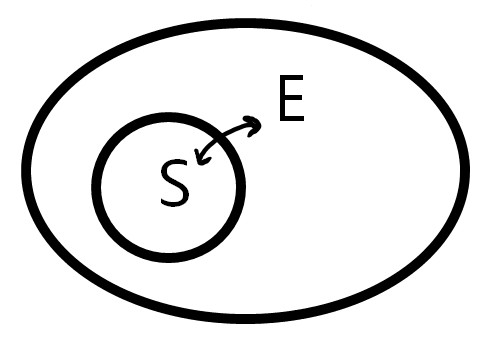
\includegraphics[width=0.5\textwidth]{2019/01/20190118_opensystem.png}
    \caption{A sketch of the sort of systems we will be interested in in this class. We have an open system $S$ which will naturally interact with its environment $E$.}
    \label{fig:opensystem}
\end{figure}
\subsection*{Classical information theory} Historically, CIT was invented in 1948 with a pioneering paper by Claude Shannon. In this paper, he asked two critical questions.
\begin{itemize}
    \item[Q1.] What is the limit to which information can be \emph{reliably} compressed?
    \item[Q2.] What is the maximum rate at which information can be reliably sent through a communication channel?
\end{itemize}
That is, we may ask about how to encode information in such a way that it can still be recovered with a high probability of success. And we can ask how to send this information when our communication channels will naturally be noisy. The answers to these questions are known as \term{Shannon's Source Coding Theorem} and \term{Shannon's Noisy Channel Coding Theorem}, respectively.

\subsection*{What is information?} We have an intuitive sense of what information means, but to formalize this takes a little work. In the loosest sense, information is associated to uncertainty and in particular information gain is related to a reduction in uncertainty.
\begin{exm}
Suppose I have a system which takes some discrete values, e.g. I roll a fair die. The outcome is a variable $x$ which takes values in some set, $J=\set{1,2,\ldots, 6}$. We write that capital $X$ is proportional to $p(x),x\in J$, where $P(X=x)=p(x)=1/6\, \forall x\in J$. That is, there is a probability mass function associated to the possible outcomes. The probability that we measure the system $X$ in outcome $x$ is $1/6$ for any outcome $x$ in the set of outcomes.
\end{exm}

We also define the following quantity.
\begin{defn}
\term{Surprisal} is the quantity
\begin{equation}
    \gamma(x)=-\log p(x).
\end{equation}
When an event is very unlikely and it happens anyway... you are very surprised. For example, $p(x)=1\implies \gamma(x)=0$ (certainties are not very surprising) while $p(x)\approx 0 \implies \gamma(x)$ large. See Fig. \ref{fig:surprisal} for a plot of $\gamma$ versus $p$.
\end{defn}
This quantity has some features:
\begin{itemize}
    \item It only depends on $p(x)$ and not on $x$.
    \item It is a continuous function of $p(x).$
    \item It is additive for independent events.
\end{itemize}
This last property is easy to prove:
\begin{equation*}
    P(X=x,Y=y)=P_{XY}(x,y)=P_X(x)P_Y(y)
\end{equation*}
when $X,Y$ are independent. Then
\begin{equation*}
    \gamma(x,y)=-\log P_{XY}(x,y)=\gamma(x)+\gamma(y).
\end{equation*}

\begin{figure}
    \centering
    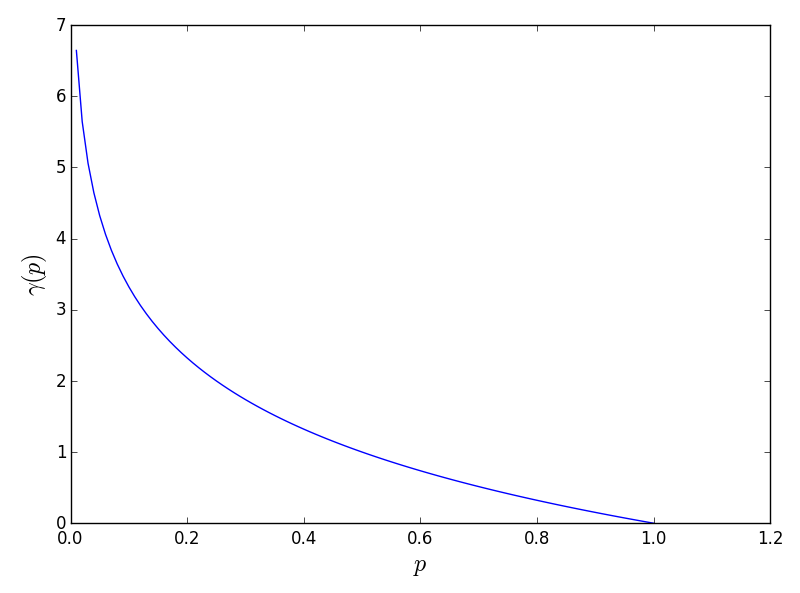
\includegraphics[width=0.5\textwidth]{2019/01/20190118_surprisal.png}
    \caption{The surprisal $\gamma(p)\equiv -\log_2 p$ as a function of $p$, the probability of some event. Certainties ($p=1$) are not very surprising, whereas very rare events ($p\ll 1$) are surprising, and so get $\gamma=0$ and $\gamma$ large respectively.}
    \label{fig:surprisal}
\end{figure}

\begin{defn}
    We can now define the \term{Shannon entropy} of $X$ to be
    \begin{equation}
        H(X)\equiv \mathbb{E}(\gamma(X))=\sum_{x\in J}(-\log p(x))p(x),
    \end{equation}
    the expected value of the surprisal. We see again that $H(X)$ does not depend on the actual outcomes themselves but only on the probability distribution $P(X)$.
\end{defn}
As a matter of convention we will take logs to be $\log{} \equiv \log_2{}$, and for events which are impossible, $P(x)=0$, we have $0\log 0 = 0$ (which one can prove by taking the limit $\lim_{u\to 0}u\log u =0$).

\subsection*{Binary entropy} Consider an event which has two possible outcomes, $X\sim P(x), x\in J =\set{0,1}$ where $P(X=0)=p$ and $P(X=1)=1-p$. Then the Shannon entropy is
\begin{equation}
    H(X)=-p\log p - (1-p)\log(1-p)\equiv h(p).
\end{equation}
We see that if the probability is $p=1/2$, then we have no information a priori about this systems-- the entropy is maximized. $h(p)$ is a continuous function of $p$, and it is concave. See the illustration in Fig. \ref{fig:binaryshannon}.

\begin{figure}
    \centering
    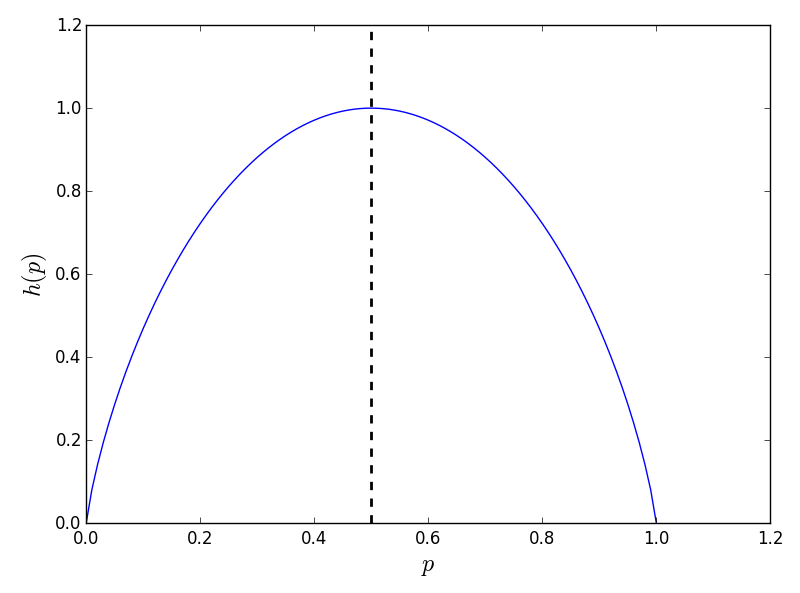
\includegraphics[width=0.5\textwidth]{2019/01/20190118_binaryshannon.png}
    \caption{The Shannon entropy of a binary event where there are two possible outcomes, one of which happens with probability $p$ and the other with $1-p$. When $p=0.5$, our ignorance is at a maximum-- we know nothing a priori about what our generator will spit out.}
    \label{fig:binaryshannon}
\end{figure}

\begin{defn}
    We can also define a different entropy, the R\'enyi entropy, which is
    \begin{equation}
        H_\alpha(X)=\frac{1}{1-\alpha}\log \paren{\sum_{x\in J}p(x)^\alpha},
    \end{equation}
    with $\alpha \in (1,2]$. As an exercise, we can verify that $\lim_{\alpha \to 1} H_\alpha(X) = H(X)$, i.e. the Renyi entropy reduces to the Shannon entropy.%
        \footnote{The proof is fairly quick. First note that as $\alpha\to 1$, the denoninator $1-\alpha$ goes to zero and the log becomes $\log (\sum_{x\in J}p(x))=\log 1 =0$, so we can apply L'H\^opital's rule and take some derivatives. Note also that $\frac{d}{dx}a^x = \frac{d}{dx} e^{\log a^x}= \frac{d}{dx} e^{x\log a} = \log a e^{x\log a}= a^x \log a$. Thus by L'H\^opital's rule,
        \begin{align*}
            \lim_{\alpha\to 1} H_\alpha(X)&= \lim_{\alpha\to 1} \frac{1}{1-\alpha}\log \paren{\sum_{x\in J}p(x)^\alpha}\\
            &= \lim_{\alpha\to 1} \frac{1}{(-1)} \frac{\sum_{x\in J} (p(x)^\alpha \log p(x)) }{\sum_{x\in J} p(x)^\alpha}\\
            &= - p(x) \log p(x) =H(X).
        \end{align*}
        Technically I have done this calculation with a natural log rather than a base 2 log, but the result is the same, since the numerical factor from taking the derivative of the log cancels with the factor from rewriting the derivative of $p(x)^a$ in terms of a base 2 log. \qed
        }
\end{defn}

Why do we choose to work with the Shannon entropy? It has to do with the operational interpretation-- the Shannon entropy represents an optimal rate of data compression, i.e. the data compression limit.

In CIT, a classical information source emits some messages/data/signals/information. For instance, $J$ could output a binary output or perhaps telegraph English (26 letters and a space). Now, the simplest class of sources is \term{memoryless}-- they are ``independent identically distributed'' sources (i.i.d.), which means that successive messages are independent of each other, and they are identically distributed.

\begin{defn}
    Suppose we have some random variables $U_1,U_2,\ldots, U_n$ with $U_i \sim p(u),u\in J$. We say these are \term{identically distributed} if
    \begin{equation*}
        p(u)=P(U_k=u), u\in J \quad \forall 1\leq k \leq n.
    \end{equation*}
\end{defn}
We could study a signal emitted by $n$ uses of the source to get some sequence $\underline{u}^{(n)}=(u_1,u_2,\ldots, u_n)$.
\begin{defn}
    Moreover, if the probability mass function takes the form
    \begin{align*}
        p(\underline{u}^{(n)}) &=P(U_1,\ldots,U_n= u_n)\\
        &= p(u_1)\ldots p(u_n).
    \end{align*}
\end{defn}

If the source is indeed independent and identically distributed, then it makes sense to describe it by a sincle probability mass function, $U\sim p(u)$, so that the Shannon entropy of the source can be said to be
\begin{equation}
    H(U)=-\sum_{u\in J} p(u) \log p(u).
\end{equation}

Another guiding question. Why is data compression possible? Our information source has some \emph{redundancy}. For instance, in the English language, certain letters are more common than others, so we can encode something that is more common in a shorter string in anticipation it will be used more often.

This sort of scheme is known as variable length coding, e.g. we might encode the letter ``e'' as the string $10$ and the letter ``z'' as $11000$. In contrast, we could also use a fixed length coding scheme where we have a ``typical set'', a subset of our total outcomes $J^n$ (things we might like to encode). Our typical set then has a one-to-one mapping to the set of encoded messages, e.g. $\set{0,1}^m$, so we can always recover them precisely, while several outcomes outside the typical set might map to the same encoded message. There's some probability that we'll want to encode things outside the typical set, and in decoding we'll get the original message a little bit wrong. But if we choose the typical set well, this can be made to be a rare occurrence. We are usually interested in \emph{asymptotic i.i.d.} settings, i.e. in the limit as the size of the set of possible messages to be encoded goes to $\infty$.

\begin{exm}
    Suppose we have a horse race with eight horses. They have labels $1,2\ldots, 8$, and the message we would like to encode is the label of the winning horse. A priori, we only need $3$ bits to encode the label since $2^n$ different messages can be stored in $n$ bits.
    
    However, what if the horses are not all equally fast (i.e. likely to win)? Suppose that $p_i$ is the probability of the $i$th horse winning, such that
    \begin{equation*}
        p_i=1/2,1/4,1/8,1/16,1/64,\ldots,1/64.
    \end{equation*}
    Now we assign the following code words:
    \begin{align*}
        C(1)&=0\\
        C(2)&=10\\
        C(3)&=110\\
        C(4)&=1110\\
        C(5)&=111100\\
        C(6)&=111101\\
        C(7)&=111110\\
        C(8)&=111111.
    \end{align*}
    Let $l_i$ be the length of the $i$th codeword, e.g. $l_5=6$. We can compute that the average length of a code is then $\sum p_i l_i = 2$, and we've chosen a ``prefix-free code'' so that a sequence like 10011001110 can be uniquely decoded to a sequence of winners from our code words. That is, no codeword is a prefix of any other code.%
        \footnote{For the sequence 10011001110, we know that the first winner was the horse corresponding to 10, horse 2. The next winner was horse 1 with code 0. This sequence breaks up as $10|0|110|0|1110$, so the winners were 2, 1, 3, 1, and 4 in that order.}
        
    Let's compute the expected length of the codeword-- it is
    \begin{equation}
        \sum_i p_i l_i=1\times \frac{1}{2}+2\times \frac{1}{4}+3\times \frac{1}{8} + 4 \times \frac{1}{16}+4 \times \frac{1}{64}\times 6=2,
    \end{equation}
    and this is exactly the Shannon entropy of the system, as expected.
\end{exm}